\documentclass[12pt,a4paper]{article}
\usepackage[utf8]{inputenc}
\usepackage[spanish]{babel}
\usepackage{graphicx}
\usepackage{kpfonts}
\usepackage[left=2cm,right=2cm,top=2cm,bottom=2cm]{geometry}
\author{Jorge Bueno}
\begin{document}
\title{Universidad Politecnica \\ de la \\ Zona Metropolitana de Guadalajara}
\author{Tarea 5\\Jorge Heriberto Bueno Gomez 18312259\\Ing. Mecatronica 4 B}
\maketitle
$$
\includegraphics[scale=.5]{UPCDLZMDG5783-logo.png} $$
\newpage
\section{Motor de corriente directa} 
El motor eléctrico es una máquina que se encargan de convertir la energía eléctrica en energía mecánica a través de la acción de los campos magnéticos producidos por sus bobinas.
Los motores de corriente directa tienen varias diferencias ya que son construidos de diferente manera comparados con los de corriente alterna. Una de las principales diferencias es que pueden funcionar a la inversa, es decir no solamente pueden ser utilizados para transformar energía eléctrica en  mecánica. También pueden funcionar como generadores de electricidad. Esto sucede por que tienen la misma construcción física que los generadores.
Los motores de corriente continua tienen un par de arranque alto comparado con los de corriente alterna, También son mas fáciles de controlar la velocidad, por tal motivo son eficaces en aplicaciones donde se requiera un control de velocidad. Son usados para ascensores, trenes, tranvías, automóviles eléctricos y todas aquellas aplicaciones en las que se requiere un control de velocidad constante.

\subsection{Inversor de giro de motor DC}
Los pulsos lentos generados por el astable LM 555 son amplificados en corriente para excitar las bobinas de los relevos los cuales forman una llave de cruce que alimenta el motor con una fuente de poder distinta a la del circuito de control.

Obviamente las bobinas de estos relés determinarán el voltaje del circuito oscilador; por otro lado los contactos del relé, la capacidad o amperaje para manejar el motor ya que esta es independiente de la parte de control//



\subsection{Para qué sirve invertir el giro en un motor monofásico}
La inversión del giro permite al motor monofásico ejercer fuerza mecánica en sentidos opuestos, aunque no de forma simultánea. Por ejemplo, se puede utilizar para elevar una plataforma para vehículos, e invertir el giro para pararla.

También se pueden emplear como elemento de ayuda para subir o bajar las ventanillas eléctricas, cuando el coche no tiene batería, y se le acopla una alimentación externa (siempre y cuando no exista una centralita que comande el conjunto).


\section{Cómo se realiza la inversión del giro en motores monofásicos}
A continuación, te presentamos los diferentes tipos de motores y cómo se realiza en cada uno de ellos la inversión del giro:\\

\textbf{Motores de fase partida:}\\
Estos son los componentes principales de los motores de fase partida:

Estator. Consiste en dos devanados o bobinas aisladas entre sí y conectadas para que formen dos devanados separados, uno principal y otro auxiliar. 
Rotor. Se trata de un núcleo en forma de cilindro de acero. Sobre su mismo eje se suele instalar un ventilador para que refrigere. 
Interruptor centrífugo. Su función principal es desconectar el devanado auxiliar una vez que el motor ya se ha puesto en marcha.
Escudos. Su misión es mantener el rotor en su sitio, evitando fricciones y rozaduras.
Carcasa. Alberga y protege el resto de elementos del motor.
En el momento del arranque el motor es bifásico, con sus devanados desfasados entre sí 90º para que se pueda poner en marcha. Cuando se alcanza el régimen de vueltas necesario se desconecta el devanado de arranque y, a partir de entonces, funciona como monofásico.

La desconexión del devanado auxiliar se realiza mediante los interruptores centrífugos situados en el eje. Los devanados están conectados en paralelo a una placa de bornes y, aparte, el devanado auxiliar se suele conectar en serie a un condensador electrolítico con la finalidad de mejorar el par de arranque y su rendimiento. Se pone en marcha de forma manual, mediante un interruptor de dos polos.

Si se quiere invertir el sentido de giro se deben invertir las conexiones de uno de los devanados en la placa de bornes, en ningún caso se deben invertir las conexiones de alimentación, porque el motor seguirá girando en la misma dirección.\\

\textbf{Motores con arranque por condensador:}\\
Al acoplar un condensador al devanado auxiliar de arranque se aumenta hasta 3 y 4 veces el par normal de giro. Por ello, se suele tratar de motores sometidos a una gran carga de trabajo: bombas, compresores, lavadoras industriales, etc.

El funcionamiento es prácticamente el mismo que el de fase partida, y por tanto la forma de invertir el giro del motor sería cambiando entre sí los terminales del devanado de arranque.\\

\textbf{Motor de espira en cortocircuito:}\\
Se trata de un motor de baja potencia, empleado principalmente en ventiladores. Está formado por un estator con polos salientes y un rotor con jaula de ardilla. Se instala una espira en cortocircuito en la masa polar, abarcando así gran parte del polo. A su vez, los devanados rodean las masas polares.

Al aplicar corriente a los devanados se crea un campo magnético. Este campo magnético no es capaz por sí mismo de arrancar el motor, por lo que la corriente que pasa por la espira crea una fuerza electromotriz inducida. Al mismo tiempo, produce un flujo propio que se opone al principal, creando así un sistema de dos flujos en el que el propio está desfasado respecto al principal, lo cual permite girar al motor.

Por tanto, el sentido de giro del motor será el que va desde el eje del polo a la espira. Si deseamos invertir el sentido de giro será necesario desmontar el motor e invertir el rotor manteniendo a su vez la posición del estator.

Al hablar del funcionamiento y constitución de motores monofásicos estamos entrando en el terreno de la electricidad, por lo que si quieres más información sobre las variantes utilizadas en automoción puedes visitar nuestro artículo sobre motores eléctricos.

\subsection{Puente H}
$$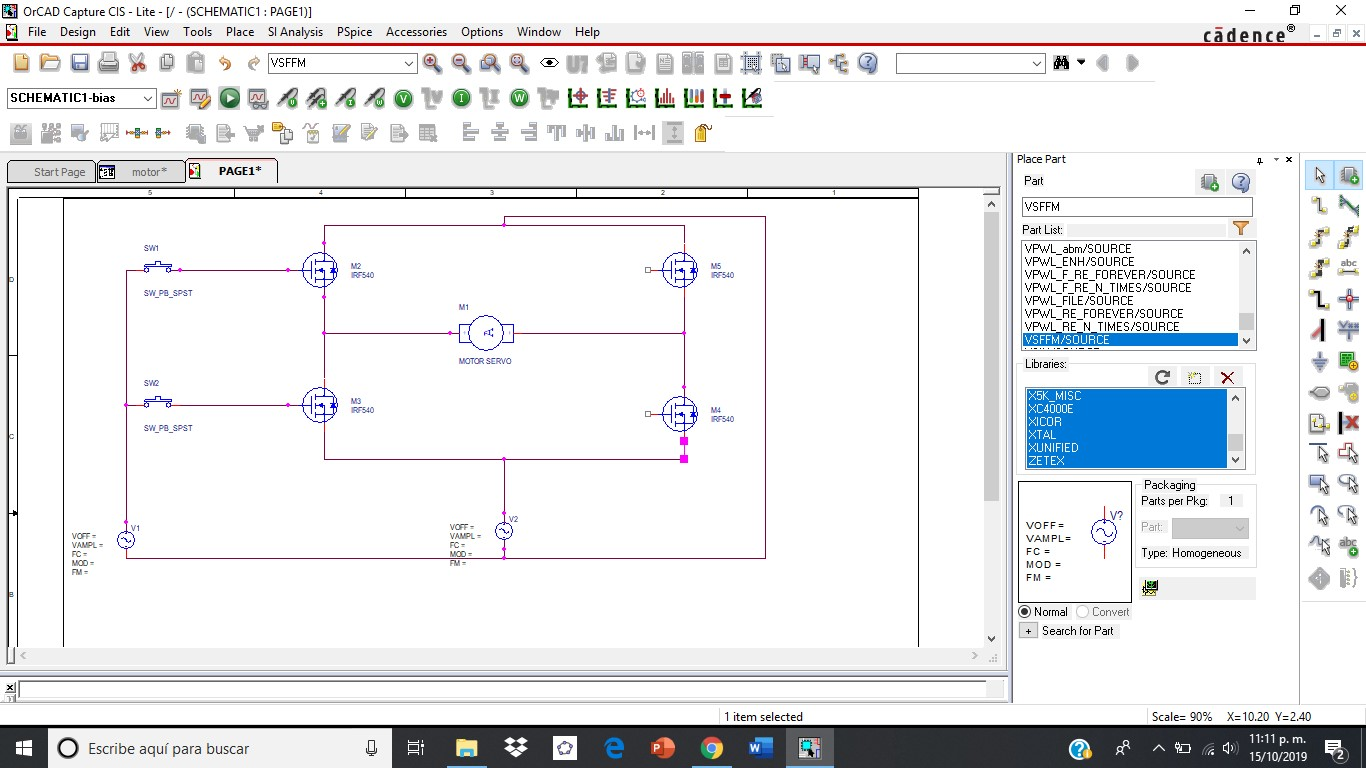
\includegraphics[scale=.4]{2.jpg} $$\\
A este tipo de circuito le llamamos puente h ya que nos ayuda a invertir el giro del motor mediante 2 swich utilizando mosfet IRF540. 
\end{document}